\subsection{Motors} \label{analysisMotors}

In this subsection, we will take a closer look at the motor. Since we chose the NXT as our platform there is only one option for our motor: the NXT motor.


The motor takes PWM as input for controlling the speed; returns the completed rotations and degrees of the next rotation.

The motor is supplied by a 9 V source. It's stalled torque is 50 N.cm, and it's stalled current is 2 A. The motor has a weight of 80g. Its maximum rotations per minute are 170, and its no-load current is 60 mA.\cite{motors}

\begin{figure}[!ht]
    \centering
	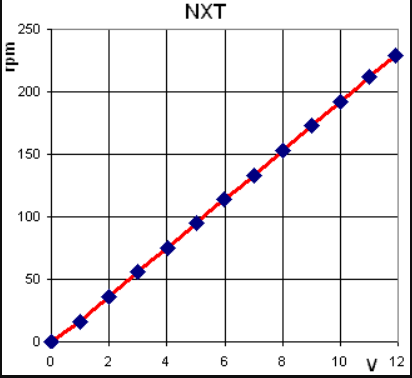
\includegraphics[width=0.7\textwidth]{Images/Analysis/nxtmotor.PNG}
    \caption{Graph of rotations per minute as a function of voltage.\cite{motors}}
    \label{fig:nxtmotor}
\end{figure}